\documentclass{easychair}



\usepackage{doc, graphicx, tikz}



\title{%
    Mikino: Induction for Dummies%
}
\author{%
    Adrien Champion%
}
\institute{%
    OCamlPro,\\%
    \email{adrien.champion@ocamlpro.com}%
}
\authorrunning{%
    Champion%
}
\titlerunning{%
    Mikino%
}



% |===| Macros
% | Names.
\newcommand{\Mkn}{Mikino}
\newcommand{\mkn}{mikino}
\newcommand{\rust}{Rust}
\newcommand{\smt}{\textsc{Smt}}
\newcommand{\bmc}{\textsc{Bmc}}
\newcommand{\smtlib}{\smt{}-\textsc{Lib}}
% | Formatting.
\newcommand{\ita}[1]{\textit{#1}}
\newcommand{\mita}[1]{\mathit{#1}}
\newcommand{\bld}[1]{\textbf{#1}}
\newcommand{\mbld}[1]{\mathbf{#1}}
\newcommand{\code}[1]{\textcolor{orange}{\texttt{#1}}}
\newcommand{\secref}[1]{Section~\ref{#1}}
\newcommand{\appref}[1]{Appendix~\ref{#1}}
\newcommand{\picwidth}{9cm}
% | Notation.
\newcommand{\vars}{\bar{v}}
\newcommand{\state}{\bar{s}}
\newcommand{\tyint}{\code{int}}
\newcommand{\tybool}{\code{bool}}
\newcommand{\init}{\code{init}}
\newcommand{\trans}{\code{trans}}
\newcommand{\cand}{\code{candidate}}
\newcommand{\true}{\code{true}}
\newcommand{\false}{\code{false}}
\newcommand{\num}[1]{\code{#1}}
\newcommand{\impl}{\Rightarrow}
% |===|



\begin{document}

\maketitle

\begin{abstract}
    \Mkn{} is a simple induction engine over transition systems. It is written in \rust{}, with a
    strong focus on ergonomics and user-friendliness. It is accompanied by a detailed tutorial
    which introduces basic notions such as logical operators and \smt{} solvers. \Mkn{} and its
    companion tutorial target developers with little to no experience with verification in general
    and induction in particular. This work is an attempt to educate developers on what a \ita{proof
    by induction} is, why it is relevant for program verification, why it can fail to (dis)prove a
    candidate invariant, and what to do in this case.
\end{abstract}

% \setcounter{tocdepth}{2}
% {\small\tableofcontents}


\section{Introduction}%
\label{sec:intro}

% \Mkn{} is a small, \smt{}-based induction engine over transition systems. It is essentially a bare
% bone version of the proof engine found in the \textsc{Kind} \(2\)~\cite{kind2} model checker.
% \Mkn{} comes with a tutorial discussing \smt{}-based induction, from \smt{} solvers to induction to
% property strengthening.

The ambition of this work is to present \smt{}-based induction to developers with no background in
formal verification. We hope to achieve this ambition thanks to our hands-on, novice-friendly
tutorial and the efforts invested in making \mkn{} as user-friendly and ergonomic as possible.
%
Note that \mkn{} is available both as a binary%
%
\footnote{%
    \url{https://github.com/OCamlPro/mikino_bin}%
}
%
and a library%
%
\footnote{
    \url{https://github.com/OCamlPro/mikino}%
},
%
which we think can motivate enthusiastic readers to try to build their own analyses.

\Mkn{} is released under \textsc{MIT}/Apache \(2.0\) (library and binary), while the tutorial
itself is under \ita{CC BY-SA} (Creative Commons Attribution-ShareAlike). We hope this encourages
teachers/trainers to use this work in relevant classes/training sessions.

The following sections discuss \mkn{}'s internals and ambitions. \appref{app:install} goes over the
process of installing \mkn{}, and \appref{app:example} illustrates \mkn{}'s input and output on
three examples. We highlight perspectives for \mkn{} in \appref{app:perspectives}.


\section{Declarative Transition Systems}%
\label{sec:input}

\Mkn{} is essentially a much simpler version of the internal proof engine found, for instance, in
the \textsc{Kind} 2~\cite{kind2} model-checker. It analyzes \ita{declarative transition systems};
such systems have a vector of typed state variables \(\vars\) that encapsulate the whole state of
the system, \ita{i.e.} no information relevant to the system exists outside of \(\vars\). For
instance, \(\vars_c = [\code{count}: \tyint,\; \code{reset}: \tybool]\). A state \(\state\) is a
valuation of the state variables, such as \(\state = [\num{7}, \false]\).

The \ita{initial state(s)} of the system are specified by a \ita{state predicate} \(\init(\vars)\):
a formula over \(\vars\). Any state \(\state\) such that \(\init(\state)\) evaluates to \true{} is
a legal initial state for the system. For instance, \(\init(\vars_c) \equiv \code{count} \geq 0
\land (\code{reset} \impl \code{count} = 0)\).
%
The \ita{transition relation} \(\trans(\vars, \vars')\) is a formula over unprimed (\ita{current})
and primed (\ita{next}) state variables. State \(\state'\) is a legal successor of \(\state\) for
the system if and only if \(\trans(\state', \state)\) evaluates to \true{}. For instance, \[
    \trans(\vars_c, \vars'_c) \quad\equiv\quad
    \code{count}' \;=\;
        \mbld{if} \; \code{reset}' \; \{ 0 \} \;
        \mbld{else} \; \{ \code{count} + 1 \}
\]
where the \ita{next} value of \(\code{count}\) is \(0\) if \(\code{reset}'\), and its old value
plus one otherwise. The next value of \code{reset} is not constrained at all.

Last, \mkn{} expects some \ita{candidate properties} or \ita{candidate invariants} which are just
called \ita{candidates}. A candidate is a predicate over \(\vars\). These candidates are named and
\mkn{} uses the name provided when producing feedback. For instance,%
%
\( \cand_1(\vars_c) \equiv \code{cnt} \geq 0 \)
%
could be a candidate for our running example.

\section{Analysis}%
\label{sec:analysis}

\Mkn{}'s analysis relies heavily on \smt{} solvers~\cite{smt}, and more precisely on Z3~\cite{z3}.
% Very roughly for space constraints, \smt{} solvers take a formula over some variables and look for
% a valuation of the variables that make this formula \true{}. If they succeed, the formula is
% \ita{satisfiable} or \ita{sat} and the solver can produce a \ita{model}: a valuation of the
% variables under which the formula \true{}. Otherwise the formula is \ita{unsatisfiable} or
% \ita{unsat} because no such model exists.
%
A \ita{proof by induction} over a transition system \((\vars, \init, \trans)\) of a candidate
\cand{} consists in showing two things:
%
\begin{itemize}
    \item \(\init(\vars) \land \neg \cand(\vars)\) is unsat,\\
        thus proving that \(\init(\vars) \impl \cand(\vars)\);
    \item \(\cand(\vars) \land \trans(\vars, \vars') \land \neg \cand(\vars')\) is unsat,\\
        thus proving that \(\cand(\vars) \land \trans(\vars, \vars') \impl \cand(\vars')\).
\end{itemize}
%
If both these formulas are unsat, then \cand{} is an invariant for the system by induction.
% This approach is slightly more technical in practice for more than one candidate, but do not
% discuss this matter further here. Note that \mkn{}'s tutorial does discuss this topic briefly,
% and readers interested in this topic can make \mkn{} log the \smt{} queries it performed to see
% exactly how it handles multi-candidate analyses ---or, alternatively, look at the code.%
% %
% \footnote{%
%     Available at \url{https://github.com/OCamlPro/mikino} and
%     \url{https://github.com/OCamlPro/mikino_bin}.%
% }

\smallskip{}

Now, if the \init{} check fails, we can extract a model from the solver. This model, by
construction, falsifies \cand{}: the candidate can be falsified by at least one of the initial
states. This is a concrete counterexamples as discussed previously.

If the \trans{} check fails however, it only means that \cand{} is not preserved by the transition
relation. This result says nothing on whether \trans{} can reach a state falsifying \cand{}. The
best we can do is to extract a model, which in this case corresponds to a pair of states \((\state,
\state')\) such that \ita{i)} \(\state\) verifies the candidate, \ita{ii)} \(\state'\) is a legal
successor of \(\state\), and \(\state'\) falsifies the candidate.

\smallskip{}

One of the main goals of the \mkn{} tutorial is to bring its intended audience of
verification-agnostic developers to fully understand what it means for a \trans{} check to fail,
and what the model extracted corresponds to. \Mkn{} itself goes to great length to have as readable
and user-friendly an output as possible, hopefully making things easier for readers going through
the tutorial.

The second main goal of the tutorial is to teach readers how to react to a failed \trans{} check.
\ita{Property strengthening} ---or \ita{candidate strengthening}, here--- consists in adding
\ita{information} to a candidate when it is not inductive. This consists in adding new candidates
that act as lemmas so that the original candidate \ita{in conjunction with the lemmas} is
inductive. The pair of succeeding states returned by failed \trans{} checks is helpful in deciding
what lemma should be added, as long as users have an understanding of what these state represent.

Strengthening can only succeed if the candidate is indeed an invariant (although a non-inductive
one) for the system. Bugs happen however, and \mkn{} can find them thanks to its Bounded
Model-Checking (\bmc{}) feature. We do not discuss \bmc{} further here, but note that on of the
\mkn{} runs shown in \appref{app:example} discusses \bmc{} and uses it to find counterexamples.


\section{Conclusion}%
\label{sec:conclusion}

\Mkn{} was created for verification novices, typically average developers, and is thus focused on
user-friendliness and ergonomics. Its companion tutorial introduces \smt{} solvers, declarative
transition systems, \bmc{}, induction, and candidate strengthening using simple terms and examples
that readers can run locally, modify, and rewrite.


\newpage{}

\label{sec:bib}%
\bibliographystyle{plain}
%\bibliographystyle{alpha}
%\bibliographystyle{unsrt}
%\bibliographystyle{abbrv}
\bibliography{bib}

\newpage{}

\appendix

\section{Installing \Mkn{}}%
\label{app:install}

\Mkn{} requires the Z3 \smt{} solver to run. In practice, this means retrieving a Z3 binary as
discussed in the tutorial:
%
\begin{center}
    \url{https://ocamlpro.github.io/verification_for_dummies/smt/index.html\#z3}
\end{center}
%
The easiest way to do this is on Z3's release page:
%
\begin{center}
    \url{https://github.com/Z3Prover/z3/releases}
\end{center}
%
By default, \mkn{} assumes the Z3 binary is in your path and called \code{z3}. You can use \mkn{}'s
\code{--z3\_cmd} to specify a different name or path. Refer to \code{mikino help} for details.
%
\\
%
We recommend you refer to tutorial's instructions for installing \mkn{}:
%
\begin{center}
    \url{https://ocamlpro.github.io/verification_for_dummies/mikino_bmc/index.html}%
\end{center}
%
which, unlike what follows, are kept updated. The easiest way to obtain the latest \mkn{} binary is
to go to its release page:
%
\begin{center}
    \url{https://github.com/OCamlPro/mikino_bin/releases}
\end{center}
%
At the time of writing, the latest version is \code{0.5.1}.

Alternatively, if \rust{} (\url{https://www.rust-lang.org}) is installed on your machine, you can
run \code{cargo install mikino} which will compile \mkn{} and put it in you path. In case you want
to update to the latest version, run \code{cargo install --force mikino}.

\section{Examples: Proof Failure/Success and \bmc{}}%
\label{app:example}

Let us go back to the example system used in the main body of this article. It is defined by its
state variables \(\vars\), its initial predicate \init{}, and its transition relation \trans{}.
We also define two candidates \(\cand_1\) and \(\cand_2\):
%
\[\begin{array}{r c l}
    \vars
        & \equiv
        & [ \code{count}: \tyint,\; \code{reset}: \tybool ]
    \\
    \init(\vars)
        & \equiv
        & \code{count} \geq 0 \land (\code{reset} \impl \code{count} = 0)
    \\
    \trans(\vars, \vars')
        & \equiv
        & \code{count}' \;=\;
            \mbld{if} \; \code{reset}' \; \{ 0 \} \;
            \mbld{else} \; \{ \code{count} + 1 \}
    \\
    \cand_1(\vars)
        & \equiv
        & \neg(\code{count} = -7)
    \\
    \cand_2(\vars)
        & \equiv
        & \code{reset} \impl \code{count} = 0
    \\
\end{array}\]

The equivalent in \mkn{}'s input format is

\begin{center}
    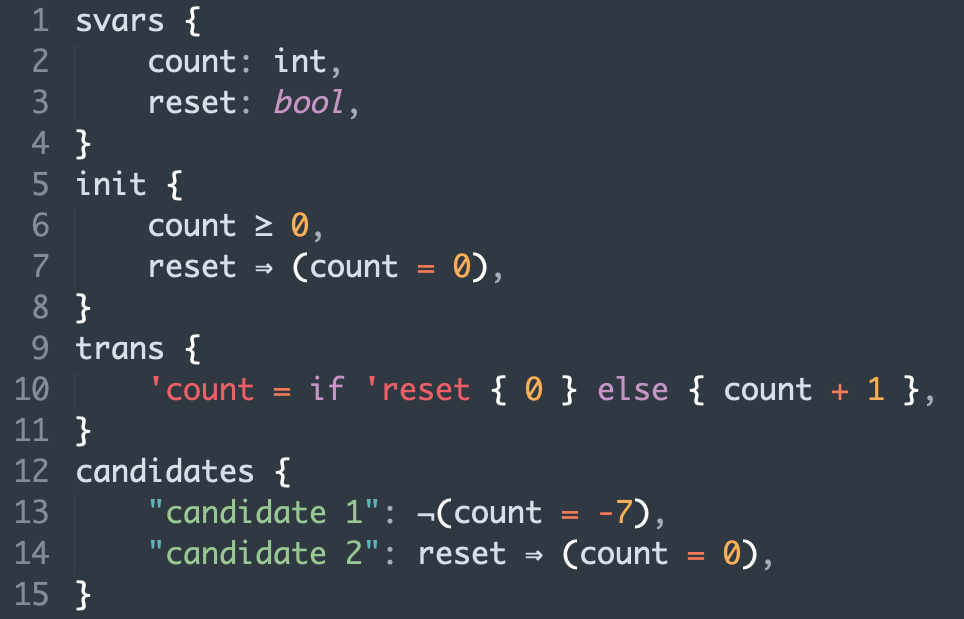
\includegraphics[width=\picwidth]{../rsc/stopwatch_1.png}
\end{center}
%
Note that:
%
\begin{itemize}
    \item \ita{primed} variables have their prime \ita{before} the identifier, not after. This is
        because we want to use Rust syntax highlighting: in Rust, \code{'<ident>} is the syntax for
        \ita{lifetimes} which make \code{'count} and \code{'reset} pop out. On the other hand,
        \code{<ident>'} would be interpreted by syntax highlighting as an identifier followed by
        the start of a character literal.
    \item \mkn{}'s Rust expressions are more readable than \smtlib{}'s S-expressions.
    \item \mkn{} supports various \textsc{UTF}-8 operators in addition to their usual \textsc{Ascii}
        equivalent(s) \code{>=}, \code{=>}, \code{\&\&}, \code{||}, \code{!}, \ita{etc.}
    \item the \init{} and \trans{} sections take a list of comma-separated expressions (with
        optional trailing comma), understood as a conjunction.
\end{itemize}

Running \mkn{} on this systems yields the following. (Run \code{mikino help} for details on
\mkn{}'s \textsc{Cli}.)
%
\begin{center}
    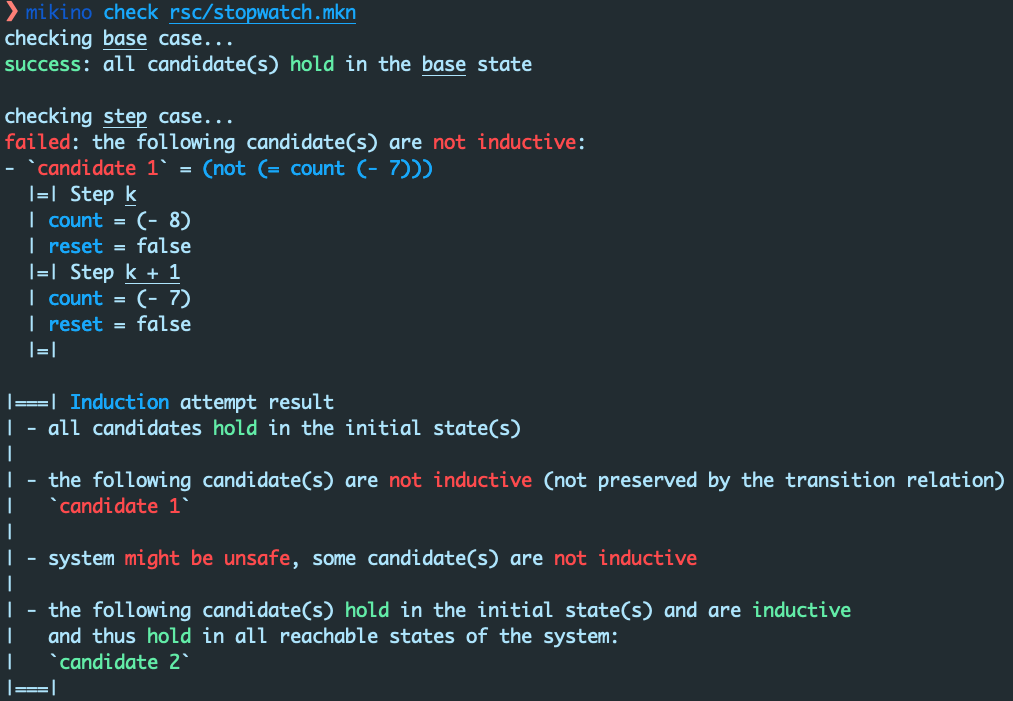
\includegraphics[width=\picwidth]{../rsc/stopwatch_run_1.png}
\end{center}
%

The first candidate is not inductive and needs some strengthening. Let us just add the very natural
lemma \(\code{count} \geq 0\).
%
\begin{center}
    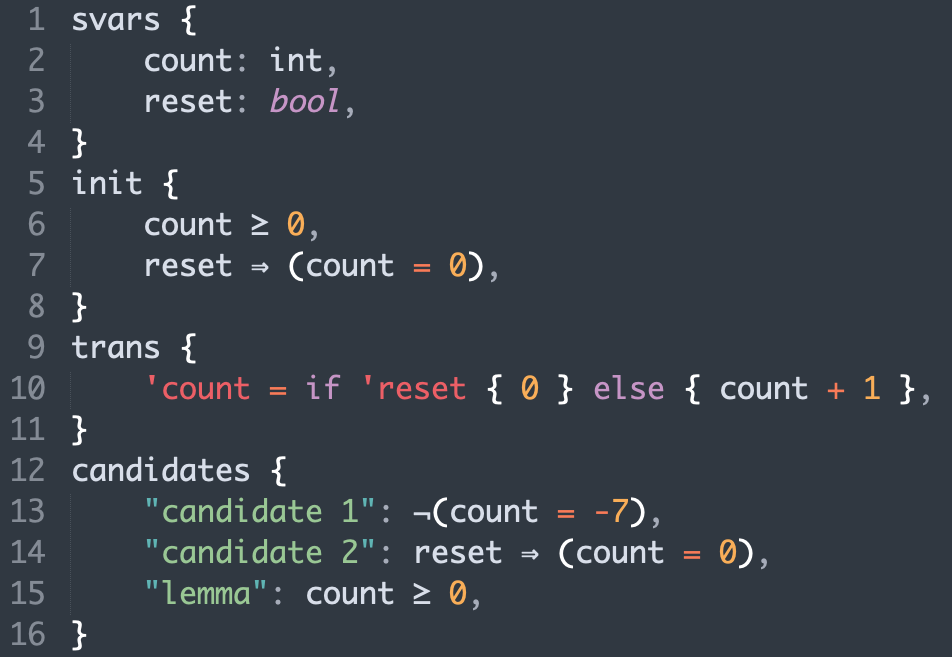
\includegraphics[width=\picwidth]{../rsc/stopwatch_2.png}
\end{center}

Running \mkn{} again, we see that the strengthening was successful and \mkn{} is able to prove all
three candidates.

\begin{center}
    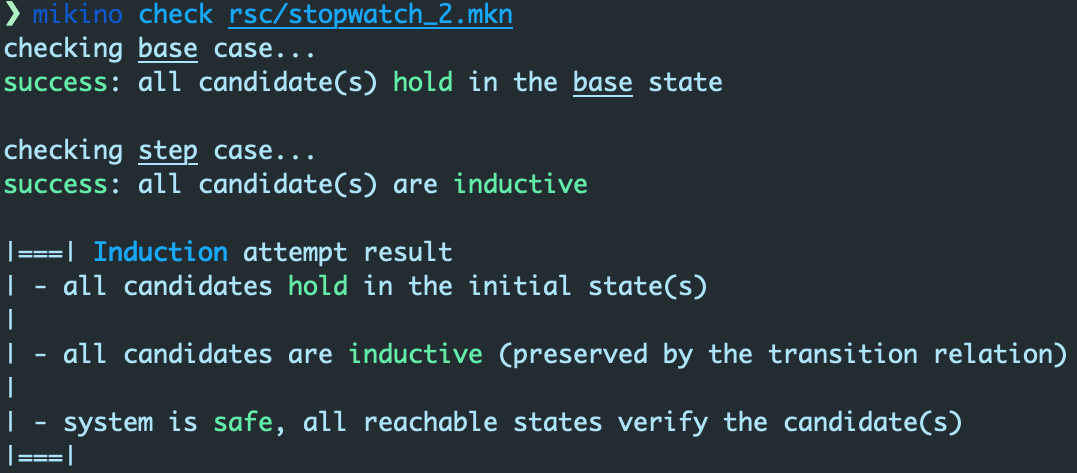
\includegraphics[width=\picwidth]{../rsc/stopwatch_run_2.png}
\end{center}

Last, here is an example of asking \mkn{} to check a falsifiable candidate by \bmc{}. 
Roughly, \bmc{} is an iterative process that starts by looking for
a falsification of the candidate(s) in the initial state, exactly like induction's \init{} check.
If none exists, \bmc{} asks the same questions about the successors of the initial states. More
precisely, is%
%
\[
    \init(\vars_0) \land \trans(\vars_0, \vars_1) \land \neg \cand(\vars_1)
\]
%
satisfiable? If it is, \bmc{} can extract a model corresponding to two succeeding states leading to
a falsification of the candidate. If not, \bmc{} \ita{unrolls} the transition relation again to
check the successors of the successors of the initial states.
%
\\
%
To showcase \bmc{} in \mkn{}, let us modify \init{} slightly and give ourselves a falsifiable
candidate.
%
\begin{center}
    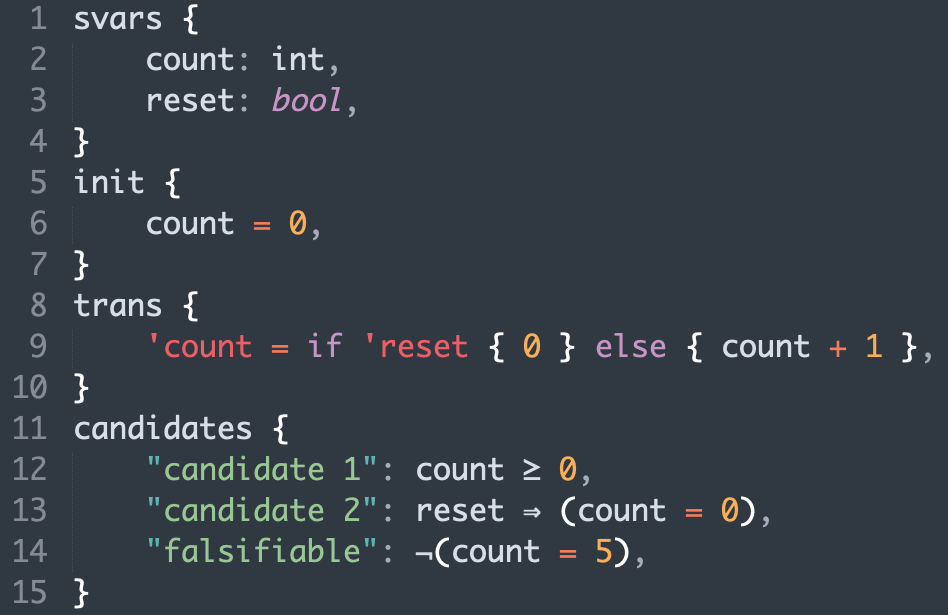
\includegraphics[width=\picwidth]{../rsc/stopwatch_3.png}
\end{center}

In \code{check} mode, \bmc{} is activated by passing the \code{--bmc} option to \mkn{}:
\code{mikino check --bmc <file>}. This option makes \mkn{} run \bmc{} on all non-inductive
candidates. The second image only shows the relevant part of the output, after the \trans{} check
counterexample is reported.

\begin{center}
    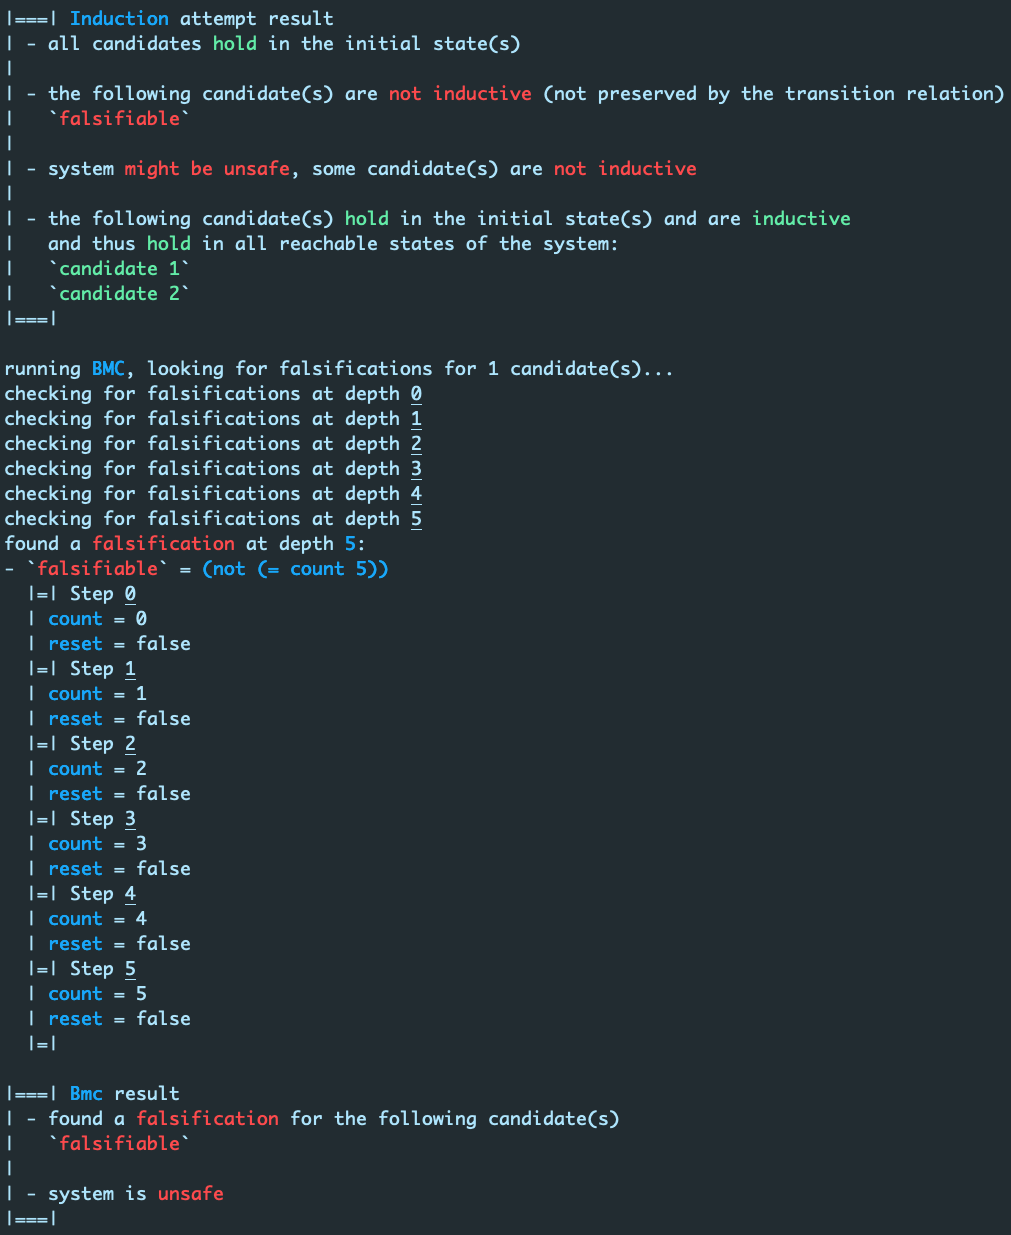
\includegraphics[width=\picwidth]{../rsc/stopwatch_run_3.png}
\end{center}


\section{Perspectives}%
\label{app:perspectives}

Since the first chapters of the tutorial go over \smt{} checks, we rely on the \smtlib{}
standard~\cite{smtlib} to write the examples. \smtlib{} is based on S-expressions as a middle
ground between human-readability and ease of parsing. While very appropriate as a common input
language for \smt{} solvers and for writing/sharing benchmarks (its main purposes), it can be
deterring for novices just starting out: \(x + 1\) for instance would be written \code{(+ x 1)}.
\Mkn{}'s syntax for transition systems is based on Rust and is much more natural to uninitiated
readers.

Depending on the feedback on \mkn{} and its tutorial, we would like \mkn{} to be able to act as a
(thin, potentially interactive) frontend for \smt{} solvers by accepting Rust-style expressions.
This would remove the need for showing \smtlib{} code at all and, we think, make it easier for
novices to dive into formal verification.



\end{document}

